\documentclass[12pt]{My_preprint}

\usetikzlibrary{arrows.meta,
                chains,
                positioning,
                shapes.geometric}
%%%%%%%%%%%%%%%%%%%%%%%%%%%%%%%%%%%%%%%%%%%%%%%%%%%%%%%%%%%%%%%%%%%%%%%%%%%%%%%
\newcommand{\size}{0.22\textwidth}
\newcommand{\avg}[1]{\left<#1\right>}
\renewcommand{\avg}[1]{\left<#1\right>}
\newcommand{\condavg}[1]{\left<#1 | \mathscr{C}_1\right>}
\newcommand{\Exp}[1]{\overline{\overline{#1}}}
\newcommand{\davg}[1]{\left<#1\right>_d}
\newcommand{\cavg}[1]{\left<#1\right>_c}
\newcommand{\Iavg}[1]{\left<#1\right>_I}
\newcommand{\pavg}[1]{\avg{\delta_\alpha #1}}
% \newcommand{\pnavg}[1]{n\left<#1\right>_p}

\newcommand{\avgcond}[1]{\left<#1\right>}
\renewcommand{\avgcond}[1]{\overline{#1}}
\newcommand{\kavg}[1]{\avgcond{#1}^k}
\newcommand{\pnnavg}[1]{\avgcond{#1}^{p}}
\newcommand{\pnavg}[1]{n_p\pnnavg{#1}}
\newcommand{\oneavg}[1]{\avgcond{#1}^1}
\newcommand{\twoavg}[1]{\avgcond{#1}^2}
\newcommand{\smallavg}[2]{\avgcond{#1}^{#2}}
\newcommand{\sym}[1]{\left(#1\right)^{\text{Sym}}}

\newcommand{\nstavg}[1]{\overline{#1}_{nst}}
\newcommand{\nstrelavg}[1]{\overline{#1}_{nst}^{rel}}
\newcommand{\mavg}[1]{\left<#1\right>_m}
\newcommand{\gavg}[2][\gamma]{\left<#2\right>_{#1}}
\newcommand{\partials}[1]{\partial_{i_1}\partial_{i_2}\ldots\partial{i_{#1}}}
\newcommand{\partialp}[2]{ \prod_{m=#1}^{#2} \partial_{i_m}}
\newcommand{\hatpartialp}[2]{ \prod_{m=#1}^{#2} \hat{\partial}_{j_m}}
\newcommand{\hatpartialpi}[2]{ \prod_{m=#1}^{#2} \hat{\partial}_{i_m}}
\newcommand{\pri}[2]{ \prod_{m=#1}^{#2} r_{i_m}}
\newcommand{\prj}[2]{ \prod_{m=#1}^{#2} r_{j_m}}
\newcommand{\nablab}{\mathbf{\nabla}}
\newcommand{\nablabh}{\nablab}
\newcommand{\nablabhI}{\nablab_{||}}
\newcommand{\ddt}{\frac{d}{d t}}
\newcommand{\pddt}{\frac{\partial}{\partial t}}
\renewcommand{\pddt}{\partial_t}
\newcommand{\norm}[1]{\hat{#1}}
\newcommand{\Jump}[1]{\llbracket #1 \rrbracket \cdot \textbf{n} }

%%% Utiliser pour les commentaires
\newcommand{\JL}[1]{\color{red}#1\color{black}}
\newcommand{\DL}[1]{\color{green}#1\color{black}}
\newcommand{\tb}[1]{\color{blue}#1\color{black}}
% \renewcommand{\alpha}{}
\renewcommand{\JL}[1]{}
% \renewcommand{\tb}[1]{}

\renewcommand{\size}[1]{0.3\textwidth}
\newcommand{\expo}[2][n]{\frac{(-1)^#1}{#1!} \partialp{1}{#1} \pavg{\int_{\Omega_\alpha} \pri{1}{#1}#2 d\Omega}}
\newcommand{\expoU}[2][n]{\frac{(-1)^#1}{#1!} \partialp{1}{#1} \pavg{\textbf{u}_\alpha\int_{\Omega_\alpha} \pri{1}{#1}#2 d\Omega}}
\newcommand{\expoS}[2][n]{\frac{(-1)^#1}{#1!} \partialp{1}{#1} \pavg{\int_{\Sigma_\alpha} \pri{1}{#1}#2 d\Sigma}}

% \newcommand{\numref}[1]{\ref{#1}}
\renewcommand{\ref}[1]{\autoref{#1}}

%%%%%%%%%%%%%%%%%%%%%%%%%%%%%%% Title & Author %%%%%%%%%%%%%%%%%%%%%%%%%%%%%%%%


\title{On the ensemble averaged stress in buoyant mono-disperse emulsion.}


\author[1,2]{Nicolas Fintzi}
\author[1]{Jean-Lou Pierson}
\author[2]{Stephane Popinet}
\affil[1]{IFP Energies Nouvelles, Rond-point de l’changeur de Solaize, 69360 Solaize}
\affil[2]{Sorbonne Université, Institut Jean le Rond ∂’Alembert, 4 place Jussieu, 75252 PARIS CEDEX 05, France}

\begin{document}

\maketitle

\begin{abstract}
    We performed direct numerical simulation (DNS) of mono disperse rising droplets. 
    This article present a numerical analysis of the pseudo turbulence Reynolds stress and interphase drag force in water / oil emulsion. 
    Indeed, in the view of feeding averaged model it is crucial to obtain course terms. 
    Until now, it wasn't possible due to the non statistically steadiness of VOF simulations because of the numerical coalescence. 
    In this work we make use of a new kind of algorithm to prevent coalescence to happen. 
    Therefor we are able to reach a statistically steady simulation and to compute the averaged closure terms. 
\end{abstract}


\section{Introduction}
\textbf{Objetcives : }

\begin{enumerate}
    \item Compute closure terms for buoyant emulsion
    \item Needs Statistically steady numerical experience to be representative 
    \item Therefore we introduce the no-calesence algorithm to obtain be statistically steady
    \item Allowing us to carry out massive DNS to compute closures terms. 
\end{enumerate}
\vspace*{1cm}
\textbf{notes}
\begin{itemize}
    \item biblio Lhuillier
    \item In the perspective of macroscopic modeling we have to close some terms 
    \begin{itemize}
        \item oil water processes
        \item vapour water process mu r = 6 
    \end{itemize}
    \item In the literature there is absolutely nothing for emulsion 
    \item Thus we study $Bo = 1$ $\mu_r = 0.1$ and $\rho_r = 1.11$. 
    \item Within the framework of hybrid model averaged equations in a mono-disperse case 
    \item Present theritical : 
     \begin{itemize}
        \item Momentum averaged equation for fluid particle two-fluid formulation. 
        \item Closure terms. (Merabahdi good intro)
    \end{itemize}
\end{itemize}
\todo[inline]{Introduce the dimensionless parameter in introduction to point out the gap for unity density and viscosity ratio. 
Do the same as \citet{hidman2023assessing}}

The configuration is also influenced by particle inertia. Citer Yin et Koch ... plus les papiers sur les ecoulements à bulles (Bunner et Tryggvason, Loisy)

Eventuellement citer quelques papiers en regime potentiel ? Discuter plus en details de la microstrucutre a la Jacques ?

Pour une sphere solide regime de Stokes on a n (R-Z) a ecrire. Pour des bulles ? experience a bas Re pour des bulles spheriques et non contaminees ?


Dans la suite il faut liste la biblio pour les differentes femetures ci apres
\subsection{Averaged forces}

\subsection{Velocity fluctutations}

\subsection{Stresslet and particle fluid particle stress}






%has a long history even in the Stokes regime. 





% \section{Modeling of dispersed two-phase flows}
% Tell that we follow the formalism of hybrid modeling for fluid particle of \citet{morel2015mathematical}

\subsection{Local scale equations}


% \section{Theoretical formulation  }

% \begin{itemize}
    \item Average procedure 
    \item Theoretical formulation of closure 
    \item Rigorous def of averaged terms 
\end{itemize}
%%%%%%%%%%%%%%%%%%%%%%%%%%%%%%%%%%%%%%%%%%%%%%%%
%%%%%%%%%%%%%%%%%%%%%%%%%%%%%%%%%%%%%%%%%%%%%%%%
\section{Numerical methodology}
How the NS equations are solved (color function etc)
\begin{itemize}
    \item Transport of the phase indicator function
    \item Single fluid formulation of momentum 
\end{itemize}
\subsection{The no-coalescence algorithm}
Objectives 
\begin{itemize}
    \item Presents the bibliography. 
    \item Introduce mani's algorithm
    \item explain step by step the algorithm
\end{itemize}


The key feature of numerical simulations is the use of a whole new algorithm which prevent numerical coalesce of droplets to occur.
First, the reader can find the described source code at \href{https://basilisk.fr/sandbox/fintzin/no-coalesce.h}{no-coalesce.h}. 
In the following we describe the global ideas and principles, then we dive into a step by step explanation of the algorithm. 
But first some worlds on the already existing algorithm is in order.

In previous studies several methods have been used to avoid coalescence. 
The first one is to increase artificially the surface tension coefficient locally such as it is done in \citet{hidman2023assessing}.
When using a level set method to track the  phase indicator function some authors developed a multiple marker level-set method to prevent coalesence, see \citet{balcazar2015multiple}. 
Similarly, for VOF tracer some author used a multi-vof approach. 
In a recent study \citet{zhang2021direct} used one VOF tracer per bubble in his simulation which prevent coalesence and allows to track bubbles independently. 
However, this approach is quite expensive as it requires solving \ref{eq:dt_alpha} for each drop. 
Instead, we adopt the methodology of \citet{karnakov2022computing} which consider a constant number of VOF tracer with respect to the number of dorplets. 
We then adoped another methodology to track bubbles independently that we adapted inside the \texttt{Basilisk} code. 

The adaptation of  \citet{karnakov2022computing} within the basilisk code has been carried out by \citet{mani2021numerical}, which developed an algorithm to prevents the adjacent droplets to have similar VOF tracers using the least VOF tracer as possible by allowing different drops to be included within the same VOF tracer.
Specifically we define $N(t)$ VOF tracer labeled as $\alpha_d^i$ for $i =0,\ldots,N$ where $N(t)$ is dependent on time since it is function of the particles positions.  
The only requirement is that the adjacent droplets at a given time $t$, have different VOF tracer to prevent coalescence. 


\begin{figure}[h!]
    \centering
    % \begin{tikzpicture}[scale=0.1,
    %     node distance = 4mm and 6mm,
    %   start chain = going below,
    %   base/.style = {draw, thick, fill=gray!10, align=center, 
    %                  inner xsep=2mm, inner ysep=2mm},
    %   rect/.style = {base},
    %   elli/.style = {ellipse, base},
    %   circ/.style = {circle, fill=graye!10, minimum size=12pt},
    %   diam/.style = {diamond, base, aspect=1.5},
    %   line/.style = {draw, rounded corners, -Stealth, semithick},
    % ]
    % % Place nodes
    % \begin{scope}[nodes = {on chain, join=by line}]
    % \node [rect, rounded corners=10pt] (step1) {start};
    % \node [rect] (step2) {(1) Apply tag function \\ on vof field $\alpha_d^i$};
    % \node [base] (step3) {(2) Check for any adjacent drops \\ that have the same $\alpha_d^i$};
    % \node [rect] (step5) {(3) Change drops vof tracers for all\\ adjacent drops.};
    % \node [diam] (step7) {$i < N(t)$};
    % \node [rect, rounded corners=10pt] (step8) {stop};
    % \end{scope}
    % % \node [rect, left=of step3] (step9) {$i = i+1$};
    % % Draw edges
    % % \path[line] (step7) -| (step9);
    % % \path[line] (step9) |- (step2);
    % %
    % \path       (step7) -- node [right,near start]{False}    (step8);
    % \node [right=of step5] {
        % };
        % \end{tikzpicture}
    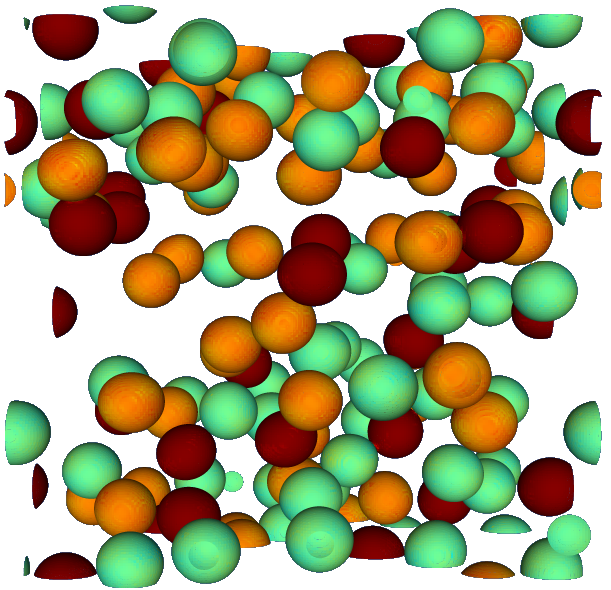
\includegraphics[width = 0.6\textwidth]{image/VOF2.png}
    \caption{
    %     Simplified flowchar of the \texttt{no-coalescence.h} algorithm.
    % $\{\alpha_d^i;i\in\mathbb{N}^{*+}\}$ represent the list of VOF tracer currently used. 
    % $N(t)$ is the total number of tracer at time $t$. 
    (b) Interface of the droplets colored by the value of $\alpha_d^i$ at $t_g =100$.
    }
    \label{fig:diagram}
\end{figure}


The simplified workflow of the algorithm follows these three steps : 
\begin{enumerate}
    \item We first identify the different topologies, i.e. the droplets, within a single tracer $\alpha_d^i$. 
    This is done by using another Basilisk feature which assign to a scalar field a different value to each topological object such as a drop (see \href{http://basilisk.fr/src/tag.h}{tag.h})\todo{biblio ?}
    \item Then we identify the droplets/tag which are different and too close to one another.
    The distance criterion is fixed to a cube of 5 mesh cells length.  
    \item Lastly we assign a new VOF tracer for each required droplets among the VOF tracer that are not already adjacent to the droplets. 
    If no VOF tracer is available we create a new one for the droplets.
    \todo{Maybe more details ?}
\end{enumerate}
This algorithm is executed at each simulation time step. 
Besides having $N$ VOF tracer require some modifications to the previously mentioned governing equations. 
Especially, instead of solving \ref{eq:dt_alpha}  we solve $N$ transport equation for each $\alpha_d^i$\todo{Is it true ?}.
But also, we compute the surface tension force as the sum of the contribution from each VOF tracer, namely, 
\begin{equation}
    \textbf{f}_\sigma \delta(\textbf{x}-\textbf{x}_I)
    = \sum_{i=0}^{N(t)} \sigma \kappa \nablab \alpha_d^i
\end{equation} 
where $\kappa_i$ is the approximate curvature of $\alpha_d^i$. 
In the 2D simulations (not presented here) we do not used more than 4 VOF tracers for hundreds of droplets during a simulation. 
This is a consequence  of the four color map theorem derived from topological arguments.
In the three-dimensional were we simulated hundreds of droplets we observed the creation of $6$ VOF tracer in the long run of the simulations.
A picture of the colored VOF is shown \ref{fig:diagram} (b) where only 3 VOF tracer is needed.
Indeed, the four color map theorem isn't valid anymore therefore the increase of VOF tracer isn't surprising anymore. 

Overall, we used an optimized multi-VOF method which allows us to compute massive DNS with approximately $6$ VOF tracers. 

\subsection{Ensemble average approximation}

Objectives : 
\begin{itemize}
    \item Present How we compute the particle properties. 
    \item Explain How we approximate the ensemble average in the numerical calculations
    \item Focus on the drag force term and on the velocity fluctuation. 
\end{itemize}

Following \citet{du2022analysis} we consider ergodicity at all time of the numerical experiment.
Thus, the ensemble average of a quantity $X$ can be approximated by a spatial average $\Xavg{X}$ and a time average $\Tavg{X}$ such that $\avg{X} = \Xavg{\Tavg{X}}=\Tavg{\Xavg{X}}$.
Consequently, the ensemble average of a numerical field, $X$, is taken through space and time such that,
\begin{equation}
    \avg{X}
    = \Tavg{\Xavg{X}}
    = \frac{1}{ t_{end} - t_0}\int_{t_0}^{t_{end}} 
    \Xavg{X}(t) dt
\end{equation}
where, 
\begin{equation}
    \Xavg{X}(t)
    = \frac{1}{L^3}\int 
    X(\textbf{x},t) d\textbf{x}
\end{equation}
where $L$ is the length of the cubic domain.
$t_0$ and $t_{end}$ is the starting time of sampling and the time duration of the simulation, respectively.
In practice, we take $t_0$ such that the simulation reach a statistically steady regime for $t>t_0$.  
Both $t_{end} $ and $t_0$ are given in \ref{ap:A} after several validations studies. 

To compute the continuous phase averaged quantities such as \ref{eq:def_uuc} we proceed as such,
\begin{equation}
    \phi_c \bm{\sigma}^{\text{Re}}_c /\rho_c
    % = \Tavg{\Xavg{\chi_c \textbf{u}_c' \textbf{u}_c'}}
    = \Tavg{\Xavg{\chi_c (\textbf{u}_c^0 -\textbf{u}_c ) (\textbf{u}_c^0 -\textbf{u}_c)}}
    = \Tavg{\Xavg{\chi_c \textbf{u}_c^0 \textbf{u}_c^0}}
    -  \phi_c  \textbf{u}_c \textbf{u}_c.
    \label{eq:def_uuc_num} 
\end{equation}
where the indicator funciton $\chi_c$ must be understood as its approximation in the DNS, i.e the color function $1 - \alpha_d$. 
Consequently, \ref{eq:def_uuc_num} indicate that we must take the average of the product of the velocities, and then we retrieve the mean velocities' product. 
Additionally,  note that the Reynolds stress can be decomposed by such as : 
\begin{align*}
    \phi_c \bm{\sigma}^{\text{Re}}_c /\rho_c
    &= 
    \Tavg{\Xavg{\chi_c (\textbf{u}_c^0 -\Xavg{\chi_c\textbf{u}_c^0} / \Xavg{\chi_c} ) (\textbf{u}_c^0 -\Xavg{\chi_c\textbf{u}_c^0} / \Xavg{\chi_c} )}}\\
    &+ \Tavg{\Xavg{\chi_c} (\Xavg{\chi_c\textbf{u}_c^0} / \Xavg{\chi_c} - \textbf{u}_c ) (\Xavg{\chi_c\textbf{u}_c^0} / \Xavg{\chi_c} - \textbf{u}_c)}\\
\end{align*}
where the first term is the space fluctuation relative to the instantaneous mean velocity of the fluid $\Xavg{\chi_c\textbf{u}_c^0} / \Xavg{\chi_c}$, and the second is the time fluctuation of the instantaneous mean velocity of the fluid. 

Similar expression can be derived for the particular phase by integrating the property over the volume of the particle which is done throught the use of the \texttt{tag.h} function, then we average on each particle at all time.




Introduce basilisk 
\subsection{Simulation set-up}
\begin{itemize}
    \item Introduce tri-periodic simulations
\end{itemize}


The \texttt{Basilisk} code has been validated numerous time in previous numerical studies \todo{Add biblio}\citet{innocenti2020direct},\citet{popinet2018numerical}. 
Therefore,  in this section we start by presenting a brief comparison with previous numerical studies. 
Afterward we present a meticulous study focusing on the interfaces dynamics, by comparing our results with the experimental results of \citet{mohamed2003drop} 
To complete these valildation we present in \ref{ap:A} several classic cases analyzing :
(1) The mesh definition, (2) The statistical time convergence, (3) the number of particles on random array of droplets. 
 
\subsection{Fixed array of bubbles}
Objectives :
\begin{itemize}
    \item Mesh validation : our DNS Vs. DNS of \cite{esmaeeli1999direct}
\end{itemize}
From our knowledge, no simulations nor experimental results have been carried out for rising buoyant viscous drop. 
Therefore, instead we reproduced the well known ordered array simulation of \citet{esmaeeli1999direct} with Basilisk to validate the mesh definition.  
It consists in a 3-D buoyant ordered rising array of bubbles. 
In our notation the flow parameters of the simulation reads, 
\begin{align*}
    \mu_r = 10,
    && \rho_r = 10,
    && Bo = 1.8,
    && Ga = 28.37,
    && \phi = 0.125.
\end{align*}
\begin{figure}[h!]
    \centering
    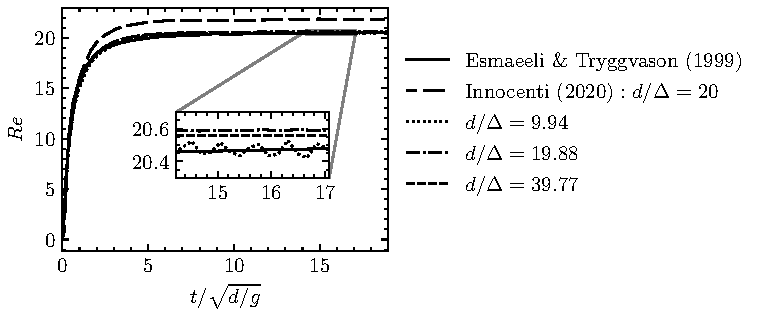
\includegraphics[height = 0.35\textwidth]{image/VALIDATION2.0/Loisy/Re.pdf}
    \caption{Time evolution of the Reynolds number based on the instentaneous volume averaged drift velocity, $Re(t) = \rho_fU d /\mu_f$, with $U(t) = (\Xavg{\textbf{u}_p} - \Xavg{\textbf{u}_c})\cdot \textbf{e}_y$ with $\phi = 0.1256$ ,$\rho_r =\mu_r =10$ and $Ga = 29.9$.}
    \label{fig:ordered_array}
\end{figure}
\ref{fig:ordered_array} display our numerical simulation against the original result of \citet{esmaeeli1999direct}
We observe very good agreements between both studies for all mesh definition.
Additionally, we displayed the results of \citet{innocenti2020direct} for $d/\Delta = 20$ to point out a divergence with our results.  
Both our simulations and the one of \citet{innocenti2020direct} have been carried out with the  \texttt{Basilisk} code. 
The cause of this difference is in fact due to a different method of interpolation used for the viscosity coefficient. 
We used an arithmetic mean, whereas \citet{innocenti2020direct} used a 
harmonic mean. 
As a matter of fact in this regime the arithmetic mean for the kinematic viscosity coefficient permit us to reach a faster convergence. 

Overall these results indicate that the criterion $d/\Delta = 30$ seems sufficient.
\todo[inline]{we could compare with bubbly flow of \citet{zhang2021direct}/\citet{roghair2011drag} \textbf{multi-vof} ? ?  }

\subsection{Drop impact on a liquid–liquid interface}
Objective : 
\begin{itemize}
    \item problematic "Do we describe well the film physics with the coalescence algorithm".
    \item Introduce the numerical set up 
    \item Comparison of the kinematic with \citet{mohamed2003drop}.  
\end{itemize}

In section we investigate in more detail the physics behind the mult-vof method. 
Indeed, we also need to check if we capture enough physics despite the fact that we do not model accurately  the film between two droplets. 
To do so we reproduced the case drop impact on a liquid–liquid interface of \citet{mohamed2003drop} as it is approximately in the range of our dimensionless numbers. 
In our notation the dimensionless parameters reads, 
\begin{align*}
    Ga = 71.02 
    && Bo = 6.40
    && \lambda = 0.33
    && \rho_r = 1.189
\end{align*}
Regarding the geometry of the problem we sceatched \ref{fig:schemeLong} the initial position of the droplet in the computational domain.
Following \citet{mohamed2003drop} we defined the dimensionless time $t / t_i = t U_i /D$ where $U_i$ is droplet velocity at $t<0$ where $t=0$ is the time of impact. 
\begin{figure}[h!]
    \centering
    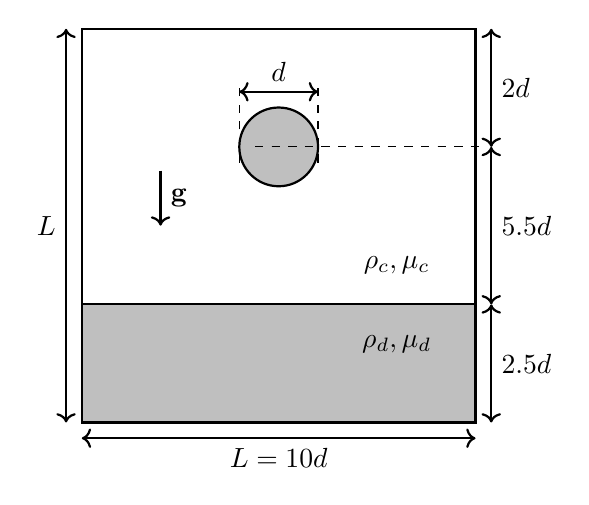
\begin{tikzpicture}[thick]
        \draw (0,0) rectangle (5,5);
        \draw[fill=gray!50] (0,0) rectangle (5,1.5);
        \draw[fill=gray!50] (2.5,3.5) circle (0.5);
        \draw[<->](0,-0.2) --++ (5,0)node[midway,below]{$L  = 10 d$};
        \draw[<->](-0.2,0) --++ (0,5)node[midway,left]{$L$};
        \draw[<->](5.2,0) --++ (0,1.5)node[midway,right]{$2.5 d$};
        \draw[<->](5.2,1.5) --++ (0,2)node[midway,right]{$5.5 d$};
        \draw[<->](5.2,3.5) --++ (0,1.5)node[midway,right]{$ 2d$};
        \draw[dashed,thin](2.2,3.5) --++ (2.9,0);
        \draw[dashed,thin](2.2,3.5) --++ (2.9,0);
        \draw[->](1,3.2) --++ (0,-0.7)node[midway,right]{$\textbf{g}$};
        \draw[<->](2,4.2) --++ (1,0)node[midway,above]{$d$};
        \draw[thin,dashed](2,3.3) --++ (0,1);
        \draw[thin,dashed](3,3.3) --++ (0,1);
        \node (a) at (4,2){$\rho_c, \mu_c$};
        \node (a) at (4,1){$\rho_d, \mu_d$};
    \end{tikzpicture}
    \caption{(left) Scheme of the computational set up at the initial time. (right) picture of the computational domain with the interfaces represented in grey.}
    \label{fig:schemeLong}
\end{figure}
\begin{figure}[h!]
    \centering
    \begin{tikzpicture}
        \node (img1) at (0,0.35\textwidth)             {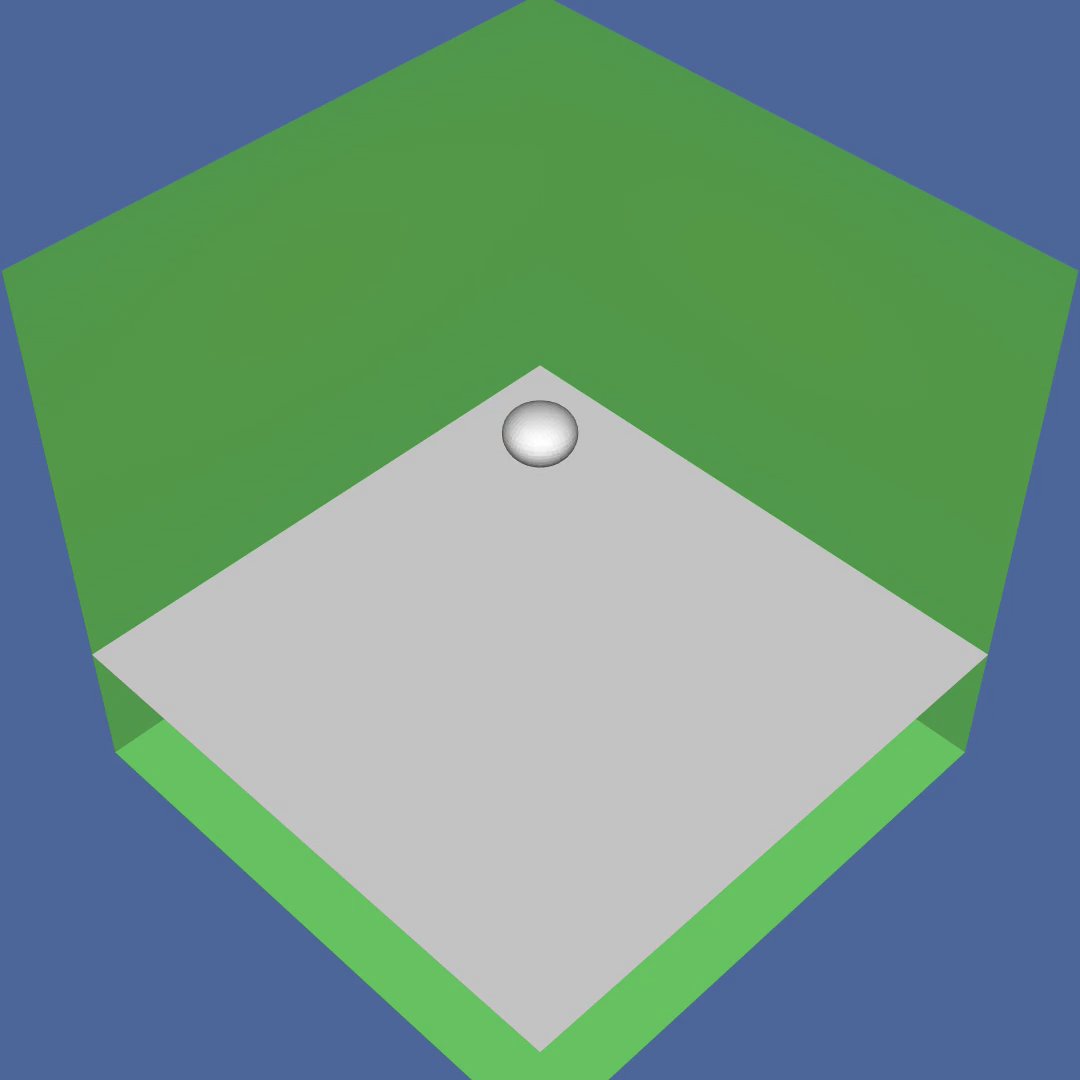
\includegraphics[height = 0.3\textwidth]{image/VALIDATION2.0/Longmire/IMG/image-010.png}};
        \node (img2) at (0.35\textwidth,0.35\textwidth) {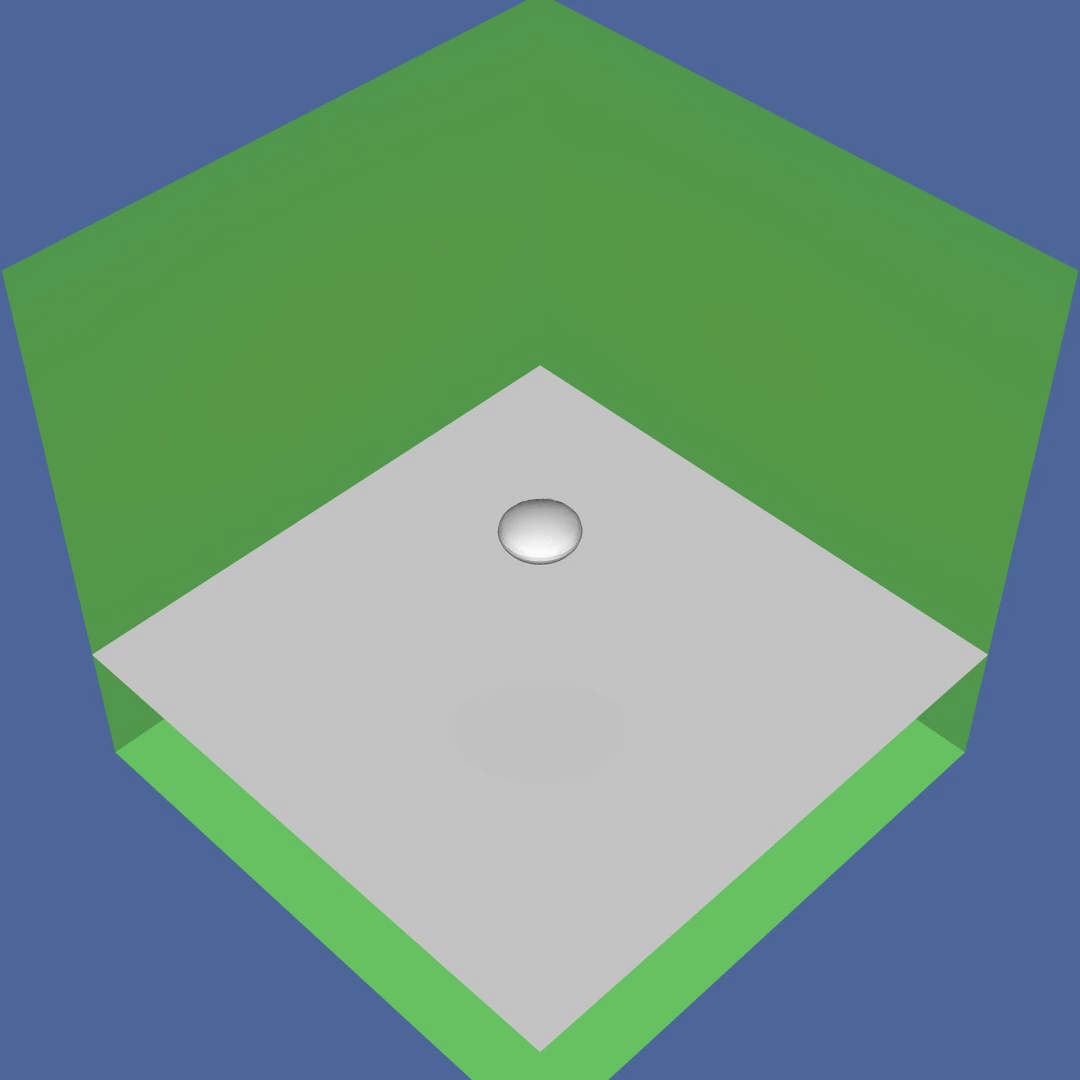
\includegraphics[height = 0.3\textwidth]{image/VALIDATION2.0/Longmire/IMG/image-020.png}};
        \node (img3) at (0.7\textwidth,0.35\textwidth) {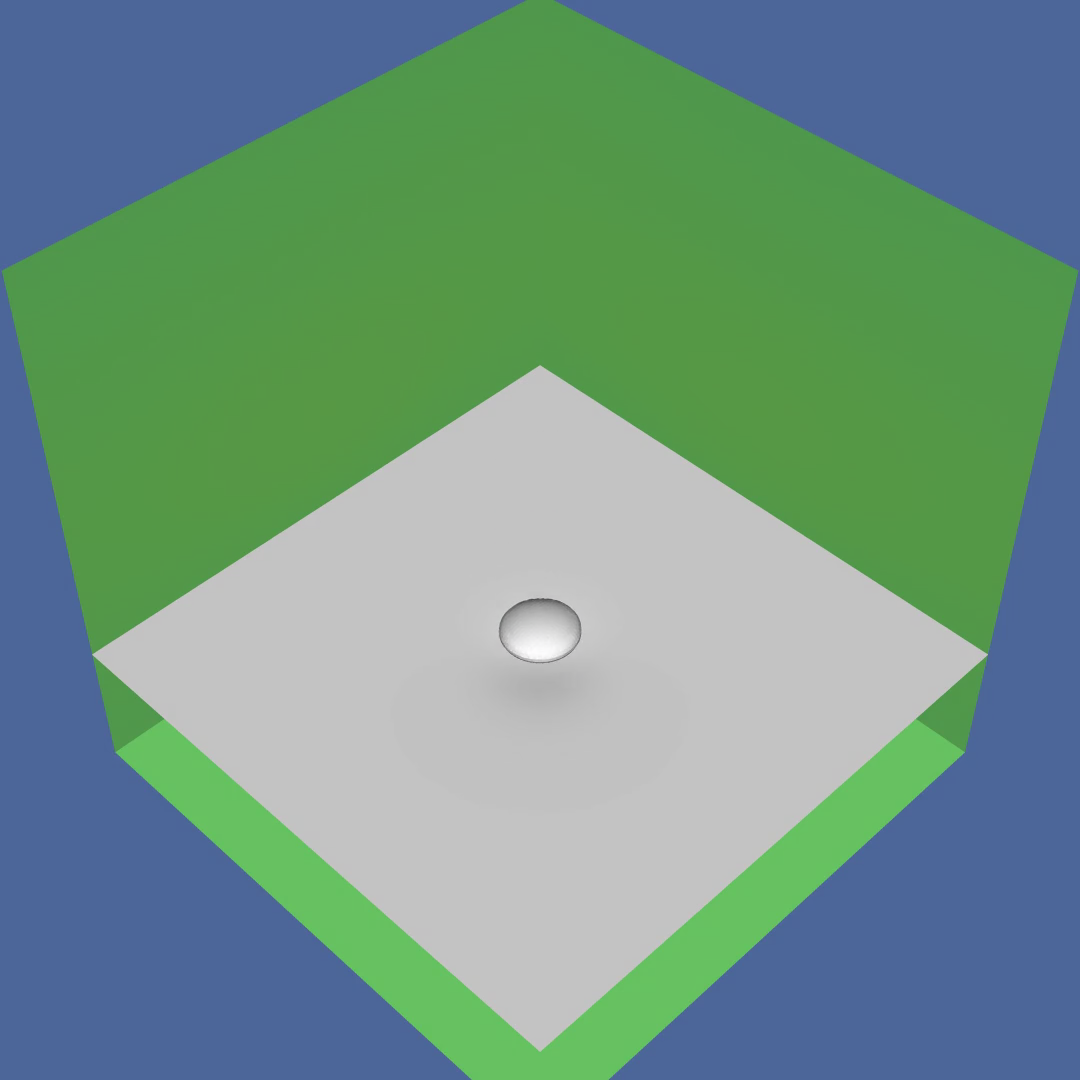
\includegraphics[height = 0.3\textwidth]{image/VALIDATION2.0/Longmire/IMG/image-030.png}};
        \node (img4) at (0,0)                         {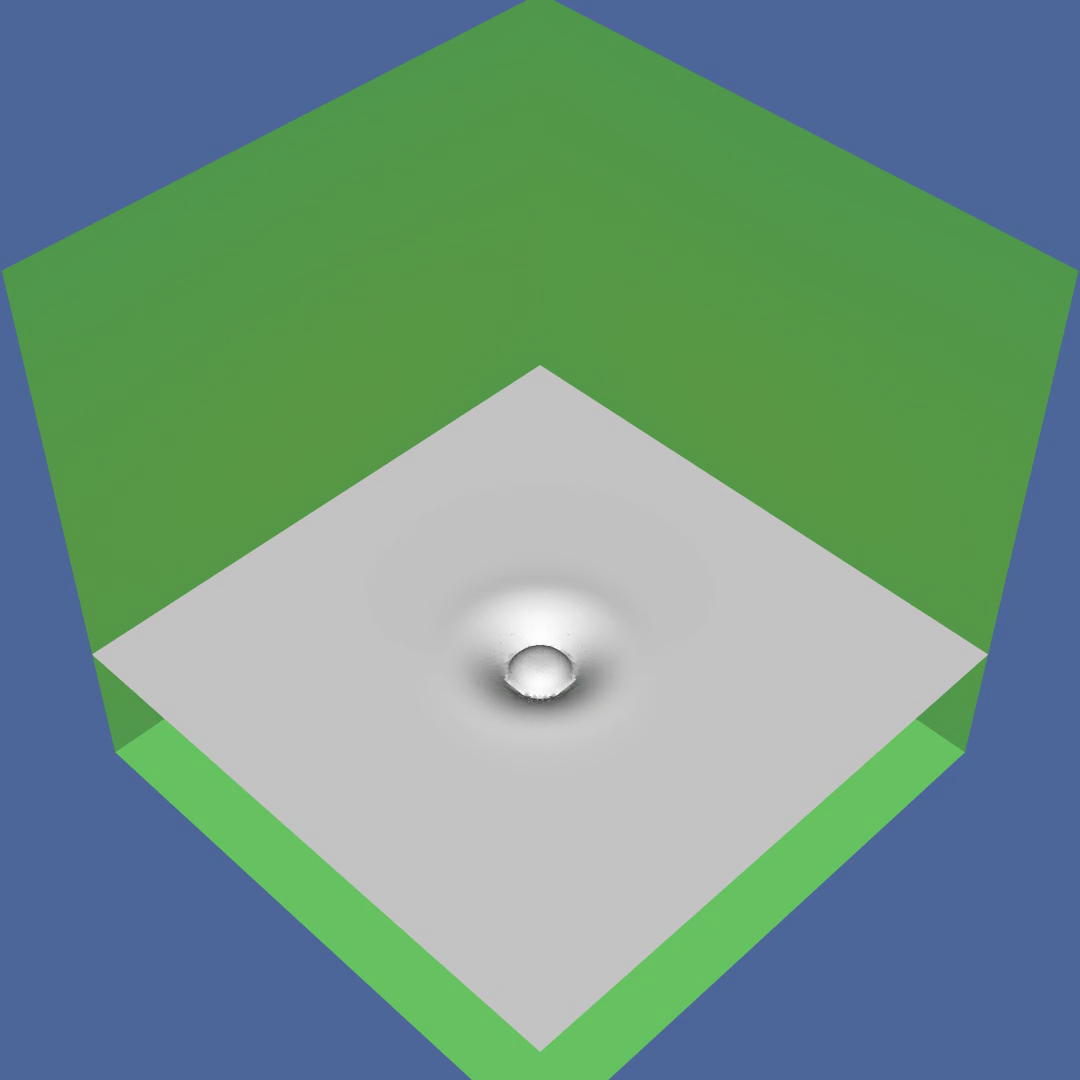
\includegraphics[height = 0.3\textwidth]{image/VALIDATION2.0/Longmire/IMG/image-040.png}};
        \node (img5) at (0.35\textwidth,0)             {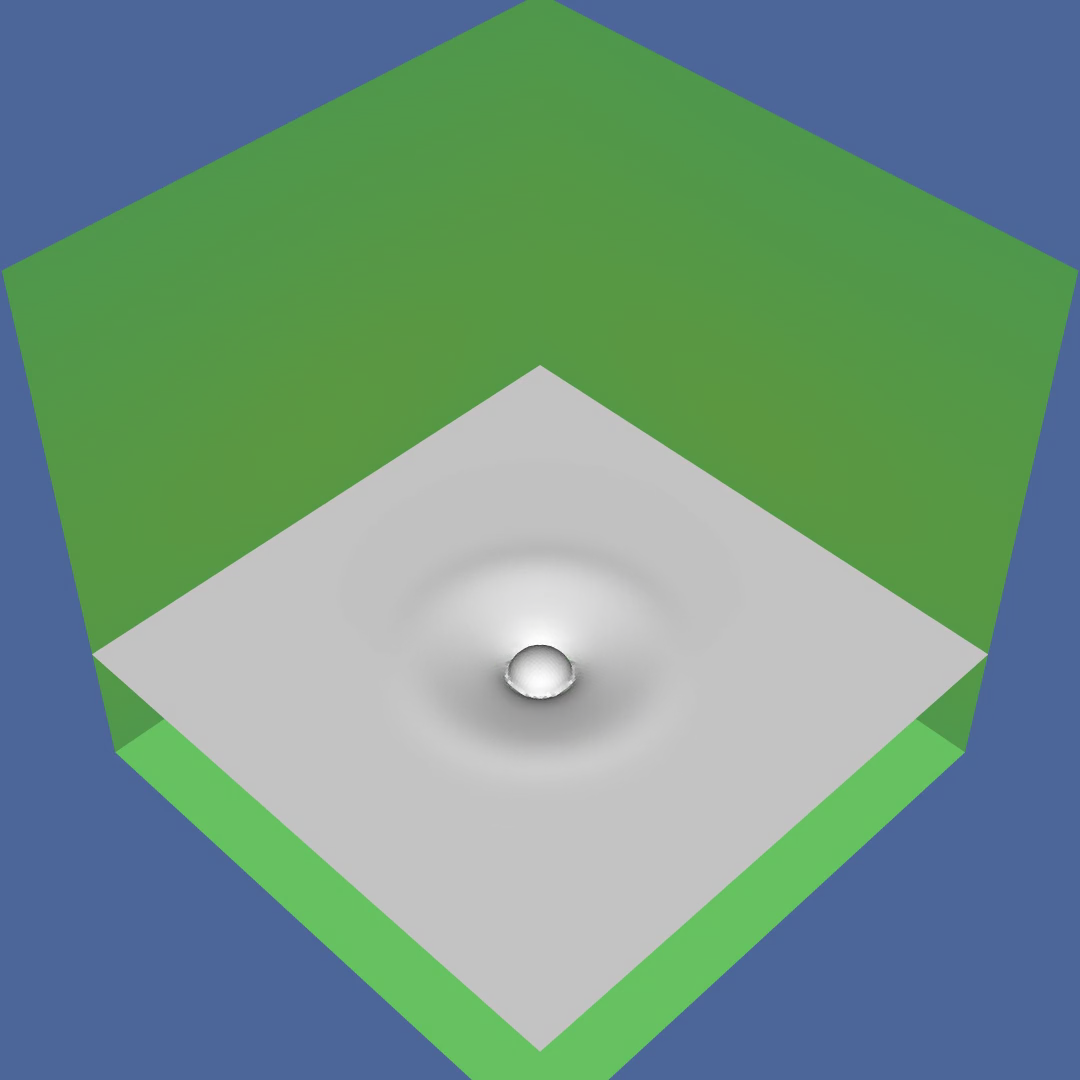
\includegraphics[height = 0.3\textwidth]{image/VALIDATION2.0/Longmire/IMG/image-050.png}};
        \node (img6) at (0.7\textwidth,0)             {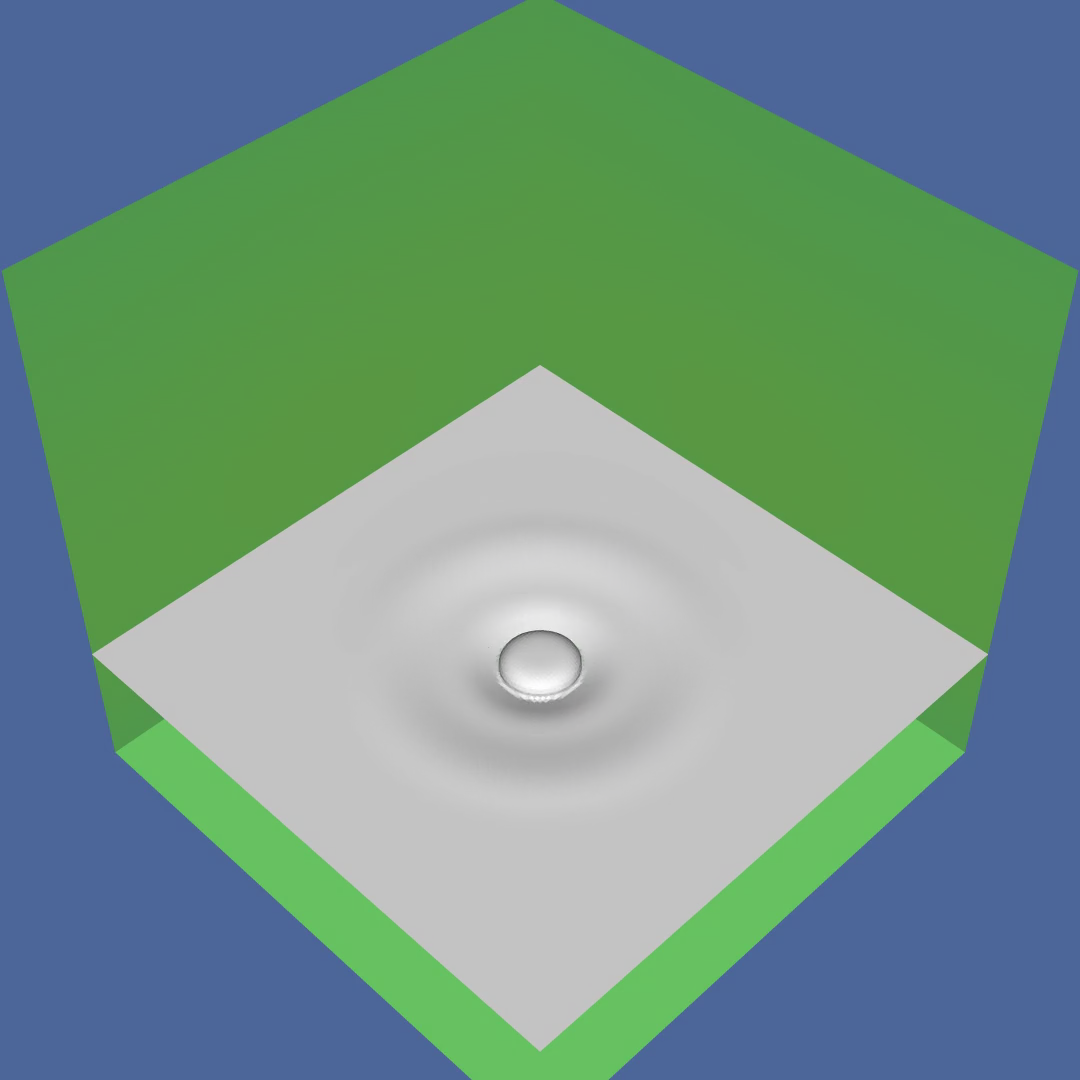
\includegraphics[height = 0.3\textwidth]{image/VALIDATION2.0/Longmire/IMG/image-060.png}};
        \node[below] at (img1.south){$t_i = -5.5$};
        \node[below] at (img2.south){$t_i = -2$};
        \node[below] at (img3.south){$t_i = 0$};
        \node[below] at (img4.south){$t_i = 2.5$};
        \node[below] at (img5.south){$t_i = 5$};
        \node[below] at (img6.south){$t_i = 15$};
    \end{tikzpicture}

    % \centering
    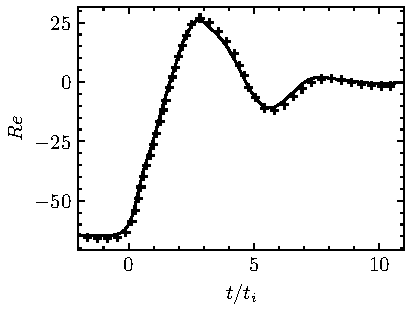
\includegraphics[height = 0.35\textwidth]{image/VALIDATION2.0/Longmire/Re.pdf}
    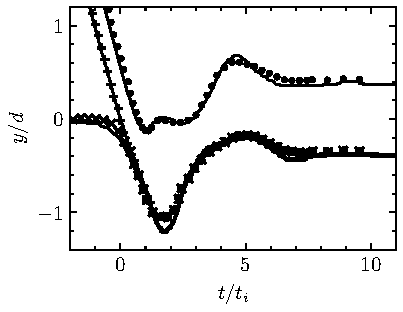
\includegraphics[height = 0.35\textwidth]{image/VALIDATION2.0/Longmire/Dist.pdf}
    \caption{(left) Time evolution of the Reynolds number based on the droplet velocity, $Re(t) = \rho_fU d /\mu_f$ in term of the dimensionless time, (+) numerical results of  \citet{balcazar2015multiple} (right)  position of the interfaces, ($\bullet$) top droplets surface, ($+$) bot droplet surface, (x) pool surface. (Symbols) experimental result of \citet{mohamed2003drop} (solid line) present numerical simulations with $d/\Delta = 30$. }
    \label{fig:resultslong}
\end{figure}
\ref{fig:resultslong} represent the comparison between our results aigainst the experiment of \citet{mohamed2003drop} (right) and the numerical simulation of \citet{balcazar2015multiple} (left). 
From the very good agreement obtained with the numerical and experimental results we conclude that the kinematic is preserved during the contact time for a mesh definition of $d/\Delta = 30$. 


%%%%%%%%%%%%%%%%%%%%%%%%%%%%%%%%%%%%%%%%%%%%%%%%
%%%%%%%%%%%%%%%%%%%%%%%%%%%%%%%%%%%%%%%%%%%%%%%%
\section{Results}
Maybe some world on the global notation of the presented results ?
\section{Average drag force}

%Objectives : 
%\begin{itemize}
%    \item Present the rising velocity Vs. phi to demonstrate the relation with $\phi^{1/3}$ \citep{loisy2017buoyancy}
%    \item Discus the common points and differences with bubbles and solid particles. 
%    \item Present a proper definition of the drag force terms such as in \citet{wang2021numerical}. 
%    \item Discus the possible correlation between the shape /arrangement of the particles/flow lines with the rising velocity. \tb{Je ne sais pas trop quoi dire la dessus}
%    \item Show that \citet{rusche2000effect}'s fit for the drag force is not adapted for our case and propose a new one
%    \item All the references for teh Drag force terms are in \citet[chap 8]{morel2015mathematical} or in \citet{ishii2010thermo}
%\end{itemize}
%\todo[inline]{include fits of bubbly flow}


%\JL{bien expliquer que ce que l'on mesure c'est les vitesses donc si on veut faire un modèle il faut repartir des vitesses (leur difference plus specifiquement). la pseudo turbulence entre elle dans la pression ou dans la viscosité ?}



%\begin{equation}
% F = ...
%\end{equation}
%On peut aussi parler du gradient de pression.


%The main difficulty is to relate the force to the flow parameters relative velocity between the two phases. 


In this section, we start by reviewing the various existing models for the averaged drag force acting on fluid inclusions in the Stokes regime. Subsequently, we consider the intermediate Reynolds number regime, the primary focus of our current investigation, proposing a drag model that reasonably fits the numerical results. As demonstrated in \ref{app:shape}, the droplet maintains an approximate spherical shape within the range of parameters studied here. Although slight deviations from sphericity are noted for $Bo=1$ and in configurations with the highest inertia, the maximum deviation from the spherical shape remains moderate less than $12$ \%. Hence, in this section we assume that fluid inclusions are spherical.

%. Henceforth, for the entirety of this section, we adopt the assumption that fluid inclusions exhibit spherical characteristics.

%Then we consider the intermediate Reynolds number regime studies which is the focus of the present work and propose a drag model which reasonably fits the numerical results. As demonstrated in Appendix \ref{app:shape} the droplet remains approximatively spherical within the range of parameters studied presently. Although some deviation from sphericity are observed for $Bo=1$ and in the highest inertial configurations the maximum deviation from the spherical shape remains moderate at around $10$ \%. Thus within the whole section, we will assume that the fluid inclusions are spherical. 


%In this section, we commence by examining existing models that describe the averaged drag force acting on fluid inclusions in the Stokes regime. Subsequently, we delve into the intermediate Reynolds number regime, the primary focus of our current investigation, proposing a drag model that effectively aligns with numerical results. As elucidated in Appendix \ref{app:shape}, the droplet maintains an approximate spherical shape within the studied parameter range. Although slight deviations from sphericity are noted for $Bo=1$ and in configurations with the highest inertia, the maximum departure from spherical shape remains modest at approximately 10%. Henceforth, for the entirety of this section, we adopt the assumption that fluid inclusions exhibit spherical characteristics.
  
%This assumption remains valid for the whole range of parameters investigated

\subsection{ The momentum balance in homogeneous sedimentation}

In the first place we would like to clarify several points about force balance and what it implies. 


\paragraph{Relation between forces and buoyancy :} The momentum conservation equations in the restricted situation of homogeneous sedimentation of particles reads from \ref{eq:dt_uc} and \ref{eq:dy_up} :
\begin{align}
    % \pddt (\phi_f\rho_f \textbf{u}_f)
    % + \div \left(\phi_f\rho_f \textbf{u}_f\textbf{u}_f + \phi_f  \bm{\sigma}_f^{\text{Re}} - n_p\textbf{M}_p \right)
    0 
    &= \phi_f 
    \left(\div \bm{\sigma}_f
    + \rho_f \textbf{g}\right)
    - n_p \textbf{f}_p, 
    \label{eq:dt_uf_steady}
    \\
    % \pddt (\phi_d\rho_d \textbf{u}_p)
    % + \div \left(\phi_d\rho_d \textbf{u}_p\textbf{u}_p+ \phi_d \bm{\sigma}_p^{\text{Re}}\right)
    0
    &= 
    \phi_d \left(\div \bm{\sigma}_f
    + \rho_d \textbf{g}\right)
    + n_p \textbf{f}_p. 
    % \label{eq:dy_up}
    \label{eq:dt_up_steady}
\end{align}
multiplying \ref{eq:dt_uf_steady} by $\phi_d$ and \ref{eq:dt_up_steady} by $\phi_f$ and subtracting the resulting equations gives, 
\begin{align}
    n_p \textbf{f}_p
    &= 
    \phi_d \phi_f (\rho_f -\rho_d ) \textbf{g}
    % \label{eq:dy_up}
\end{align}
In  mono-disperse suspension of droplets $n_p = \phi_d / v_p$ with $v_p =4/3\pi d^3/8$ the volume of a particle which yields the final results, 
\begin{equation*}
    \textbf{f}_p
    = 
    \frac{4}{3}\pi\frac{d^3}{8}\phi_f (\rho_f -\rho_d ) \textbf{g}
    \label{eq:drag}
\end{equation*}
It is convinient to make dimensionless this force with Hadamard-Ribczynski formula, which is, 
\begin{equation*}
    \textbf{f}^0_p = \pi \mu_f d A \textbf{u}_{pf}
\end{equation*}
Dividing one by the other gives the dimensionless force
\begin{equation*}
    \textbf{f}^*_p 
    = 
    \frac{4}{3A}\frac{d^2 \phi_f (\rho_f -\rho_d ) \textbf{g}}{8 u_{pf}\mu_f}
\end{equation*}
This can be made dimensionless with $\phi_f$



\paragraph{Relation between buoyancy and drag coefficient :}
We assume that the force can be written in the form, 
\begin{equation*}
    \textbf{f}_p = C_d  \pi \rho_f \frac{d^2}{8} u_{pf}^2
\end{equation*}
where $C_d$ is a dimensionless coefficient and $\textbf{u}_{fp}$ is the relative phase velocity. 
Using \ref{eq:drag} we show that $C_d$ coefficient is related to the relative velocity with, 
\begin{equation*}
    C_d  
    = 
    \frac{4}{3}
    \frac{d \phi_f (\rho_f -\rho_d ) \textbf{g}}{\rho_f u_{pf}^2}
\end{equation*}
This can be directly computed into our DNS. 
\begin{equation*}
    C_d  \phi_f^2 \frac{\rho_f^2 d^2 u_{pf}^2}{\mu_f^2}
    = 
    \frac{4}{3}
    \phi_f^3 
    \frac{
        d^3
        \rho_f
        (\rho_f -\rho_d ) g
    }{\mu_f^2}
\end{equation*}
Let us define the Galileo number as $Ga^2 = \frac{
    d^3
    \rho_f
    (\rho_f -\rho_d ) g
}{\mu_f^2}$ and the Reynolds number based on the drift velocity as, $Re =  \phi_f \frac{\rho_f d u_{pf}}{\mu_f}$,
Then, the relation between the Reynolds and Galileo is given by, 
\begin{equation*}
    Re
    = 
    Ga
    \sqrt{\frac{4\phi_f^3}{3 C_d}}
\end{equation*}
This the relative velocity is given by, 



In stokes and dilute regime the $C_d$ noted $D_c^0$ is given by Hadamard-Ribczynski solution and reads, 
\begin{equation*}
    C_d^0 = \frac{8}{Re} \left(\frac{3\lambda +2 }{\lambda +1}\right)
    = \frac{8}{Re}A
\end{equation*}
where we introduced the constant $A = \left(\frac{3\lambda +2 }{\lambda +1}\right)$. 
Thus, the Reynolds number obtained for a given \textit{Galileo} number in stokes regime is, 
\begin{equation*}
    Re^0
    = 
    \frac{Ga^2}{6 A}
    % \phi_f^3  
\end{equation*}
Since this is valid for an isolated particle we fixed $\phi_f=1$, this will be our renormalization constant. 
\begin{equation*}
    Re^*
    = 
    \frac{6A}{Ga}
    \sqrt{\frac{4\phi_f^3}{3 C_d}}
\end{equation*}
 
\paragraph{Relation between Galileo and Reynolds numbers :}
From the two previous expressions we can write the equality, 
\begin{equation*}
    \textbf{f}_p = C_d  \pi \rho_f \frac{d^2}{8} u_{pf}^2
\end{equation*} 
The hadamar ribinsky formula reads, 
\begin{equation*}
    \textbf{f}_p^0 =\pi \mu_f d A \textbf{u}_{pf}
\end{equation*}
dividing one by the other and by $\phi_f^2$ gives directly, 
\begin{equation*}
    \textbf{f}_p^* =   \frac{C_d  Re}{8 A \phi_f} 
\end{equation*}

\paragraph{Relation between dimensionless force and drag coefficient}

The hadamar-


\subsection{Stokes flow regime}

%From an experimental point of view it appears to be very challenging at most to measure the force acting on rising fluid particles in moderately dense regimes and relate it to the kinematic properties of the fluid and the particles. However, one may easily measure the mean settling or rising velocity of a suspension by measuring the velocity of its front \citep{guazzelli2011}. The mean velocity of fluid particles settling or rising in a finite vessel is known to be hindered, \textit{i.e.} to decrease with respect to the velocity of the isolated particle. Indeed the presence of a fixed bottom in a container leads to a zero velocity for the entire suspension (fluid + solid). Hence as the drops move upward, the fluid must move downward to compensate for the motion of the inclusions. This results in a decrease in the rising speed of the drops. It is usual to write this hindered velocity as  

From an experimental standpoint, quantifying the force exerted on ascending fluid particles in moderately dense conditions and establishing its correlation with the kinematic properties of both the fluid and the particles poses considerable challenges. Nonetheless, a feasible alternative involves measuring the mean settling or rising velocity of a suspension by measuring the velocity of its front \citep{guazzelli2011}. In a confined vessel, the mean velocity of fluid particles undergoing settling or rising is known to be hindered; that is, it decreases in comparison to the velocity of an isolated particle. The presence of a fixed container bottom induces a zero velocity for the entire suspension (comprising both continuous and dispersed phases). Consequently, as the droplets ascend, the fluid must move downward to counterbalance the motion of the inclusions, resulting in a reduction of the rising speed of the droplets \citep{guazzelli2011}. This hindered velocity is usually expressed as

%This decrease arises due to the presence of a stationary bottom in the container, causing the entire suspension (comprising both continuous and dispersed phases) to have a zero velocity \citep{guazzelli2011}. Consequently, as the droplets ascend, there is a compensatory downward movement of the fluid to counterbalance the motion of the inclusions, resulting in a reduction in the ascent speed of the droplets. This hindered velocity is conventionally expressed as...

%From an experimental standpoint, quantifying the force acting on ascending fluid particles in moderately dense conditions and establishing its correlation with the kinematic characteristics of both the fluid and particles poses considerable challenges. However, a more accessible metric involves determining the mean settling or rising velocity of a suspension by observing the velocity of its leading edge \citep{guazzelli2011}. In a confined vessel, the mean velocity of fluid particles settling or rising is recognized to be impeded, signifying a decrease relative to the velocity of an isolated particle. The presence of a fixed container bottom induces a zero velocity for the entire suspension (comprising both fluid and solid components). Consequently, as the droplets ascend, the fluid must descend to counterbalance the motion of the inclusions, resulting in a reduction of the rising speed of the droplets. This hindered velocity is conventionally expressed as


\begin{equation}
\frac{u_d}{u_0} = f(\phi)
\end{equation}
where $u_0$ is the rising speed of an isolated fluid inclusion and $f$ is a decreasing function of $\phi$. For fluid inclusion, in the Stokes regime ($Re=0$) the drag force is given by the Hadamard-Ribczynski formula $ F = -3\pi \mu d u_d (2/3+\lambda)/(1+\lambda)$. %drag coeficient is given by the Hadamard-Ribczynski formula 
Balancing this force with the buoyancy force one obtained the settling velocity of  spherical droplet in the Stokes regime

%\begin{equation}
%C_D = \frac{8}{Re} \left( \frac{2+3\lambda}{1+\lambda} \right)
%\end{equation}


\begin{equation}
    u_0
    = (\rho_c - \rho_d)\frac{g d^2}{18\mu_c}\left(\frac{1+\lambda}{2/3 + \lambda}\right),
    \label{eq:u_o}
\end{equation}
Hence a bubble rises 3/2 faster than a very viscous drop (or a solid sphere) of the same radius and density, the liquid properties being the same in each case.

The functional form of $f$ is much more complicated to obtain since it depends on both the microstructure and on the viscosity ratios. Specifically, for a dilute structure array consisting of a periodic arrangement of spherical inclusions, $f(\phi) =(1 - (2/3+\lambda)/(1+\lambda))a\phi^{1/3})$ where $a$ is a constant with a weak dependence on the specific form of the array \citep{sangani1987}. The decrease slope in velocity depends on $\lambda$. Indeed, the coefficient multiplying $c^{1/3}$ for a bubble ($\lambda=0$) is 2/3 of that for a solid particle ($\lambda \to \infty$). This is to be expected since this estimation is derived from the method of reflection and the aforementioned observation regarding the relative velocities of bubbles and solid particles. In contrast for random free array the function $f$ can be expressed as  $f(\phi) = (1-b(\lambda)\phi)$ where $b$ is a function approaching the value $6.5$ for large $\lambda$ and $4.5$ for small $\lambda$ \citep{wacholder1973,haber1981}. Once again, the rate of decrease is lower for bubbles compared to solid particles. We may also observe that the decrease of velocity as function of $\phi$ is much more pronounced for a structured array of inclusions compared to a random array. Hence the decrease of speed depends on the assumption made regarding the microstructure of the suspension \citep{davis1985}. In particular, rising bubbles at moderate Reynolds numbers show horizontal alignment of bubble pairs \citep{bunner2002,yin2006} which may suggest the use of a law designed for ordered microstucture. Interestingy, \citet{loisy2017} observed a decrease of the suspension velocity in $\phi^{1/3}$ in similar regime of Reynolds number. 

%The determination of the functional form of fff presents a heightened level of complexity due to its dependence on both microstructural features and viscosity ratios. Specifically, for a dilute structure array consisting of a periodic arrangement of spherical inclusions, f(ϕ)f(\phi)f(ϕ) is defined as (1−(2/3+λ)/(1+λ))aϕ1/3)(1 - (2/3+\lambda)/(1+\lambda))a\phi^{1/3})(1−(2/3+λ)/(1+λ))aϕ1/3), where aaa represents a constant with a weak dependence on the specific form of the array, as detailed by Sangani et al. (1987) \citep{sangani1987}. It is noteworthy that the diminution of velocity is contingent upon the parameter λ\lambdaλ, with the coefficient multiplying ϕ1/3\phi^{1/3}ϕ1/3 for a bubble being 2/32/32/3 times that for a solid particle. This alignment is anticipated, given that this estimation is derived from reflection methods and the aforementioned observation regarding the relative velocities of bubbles and solid particles.

%Conversely, for a random free array, the function fff can be expressed as f(ϕ)=(1−b(λ)ϕ)f(\phi) = (1-b(\lambda)\phi)f(ϕ)=(1−b(λ)ϕ), where bbb is a function converging towards 6.56.56.5 for large λ\lambdaλ and 4.54.54.5 for small λ\lambdaλ \citep{wacholder1973,haber1981}. Once again, it is evident that the rate of decrease is more gradual for bubbles compared to solid particles. Additionally, the reduction in velocity as a function of ϕ\phiϕ is more pronounced for a structured array of inclusions compared to a random array. Consequently, the deceleration of speed is contingent upon the assumptions made regarding the microstructure of the suspension \citep{davis1985}. Specifically, the ascent of bubbles at moderate Reynolds numbers exhibits the horizontal alignment of bubble pairs \citep{bunner,Yin}, implying a ϕ1/3\phi^{1/3}ϕ1/3-dependent velocity reduction, as recently observed by Loisy.



%and as mentionned above the force on an isolated bubble is 2/3  

%the term multiplying

% while for a random free array (see for instance Saffman for a discussion). The question of the microstructure in a suspension of settling particle is still open (citer Davis ...)



The results presented above are limited to very dilute configurations ($\phi \lesssim 5 \%$). However, in practical applications and especially in liquid-liquid extraction the volumic fraction of the dispersed phase can be as high as $20\%$. To adress moderately dense regimes, the current engineering approach involves resorting to empirical correlations such as the one developed by Richardson and Zaki  \citep{richardson1954}
%The current engineering practice, to obtain results in moderately dense regimes is to rely on empirical correlation such as the one developed by Richardson and Zaki  
\begin{equation}
f(\phi) = (1-\phi)^n
\label{eq:Richardson} 
\end{equation}
For solid spherical particles \citet{brzinski2018} have shown using data from 15 different studies drawn from the literature that $n$ is well approximated by $n\approx 4.5$. This approximation holds from very dilute regimes to dense regimes. As demonstrated in dilute flow there is a priori reason for this coefficient to be applicable to arbitrary viscosity ratios. \citet{ishii1979drag} by compiling various experiments found in the literature proposed values of $n\approx 3$ for bubbles and $n \approx 4$ for droplets. Hence, as in dilute flows the hindrance of the rising velocity is more pronounced for very viscous drops than low viscosity ones. To address this effect, we suggest the following correlation%To take into account this effect we propose the following correlation 

%As in diltute flows, an increase in the particle voulme fraction will make hinder
%there is a priori no reason for this coefficient to be valid for arbitrary viscosity ratio. 

%In this work we propose the following coefficient %In the most dilute configuration Wacholder oberseved a decrease of .... 

\begin{equation}
n(\lambda) = 4.5\left(\frac{2/3+\lambda}{1+\lambda}\right)
\label{eq:n}
\end{equation} 
which matches well the expressions proposed by \citet{brzinski2018} and \citet{ishii1979drag} in the limit of high and low viscosity ratios, respectively. There exist very few numerical results to validate this prediction. \citet{mo1994} have considered the fall of 16 drops within a tri-periodic box, revealing a coefficient $n$ slightly larger than in Equation \ref{eq:n} (details omitted here). The exact cause of this discrepancy remains uncertain and could stem from the slow decrease of the velocity perturbation in the Stokes flow regime. Indeed, special treatment are essential in this regime to ensure that the numerical results are independent from the number of inclusions \citet{mo1994}.

%There are very few numerical results to validate this prediction. \citet{mo1994} have considered the fall of 16 drops in a tri-peridoci box and found a coefficient $n$ slightly larger than equation \ref{eq:n} (results not shown here). We do not know the exact reason of this discrepancy which may be due to the slow decrease of the velocity perturbucation in the Stokes flow regime which require special treatment in the Stokes flow regime to make sure that the results are independent on the number of inclusions. %trestament of periodic interactions %Even if for Stokes flow  
%Indeed even in very diulte regime the hindered settling velocity is a function of $\lambda$.
Our focus has been exclusively on the upward velocity of a droplet suspension. Can this information be related with the mean drag force experienced by the droplets? In the Stokes regime, the answer is affirmative. This is emphasized in the book of \citep{jackson2000}, and we draw a similar line of reasoning for ascending droplets. By eliminating the pressure gradient in the equations \ref{eq:uf_triperio} and \ref{eq:up_triperio}, we obtain the force acting on the droplets as

%Up to know we have focused our attention entirely on the rising velocity of a suspension of drop. Is this information may be related to the mean drag force acting on the drops ? the answer is yes in the Stokes regime. This is empahsized in the book of \citep{jackson} and we present here a similar reasoning for rising drops. Eliminating the pressure gradient in equations ... we obtain the total force on the drops 
%This is emphasized in the book of Jackson but we repeat here for the sake of completness. 
\begin{equation}
nf_p = \phi(1-\phi)(\rho_d -\rho _c)g
\label{eq:bdf}
\end{equation}
where $nf_p$ is the vertical component of $n\mathbf{f_p}$. Due to the linearity of the Stokes equation the force per unit of volume may be expressed as $nf_p = A (u_c -u_d)$ where $u_c$ and $u_d$ are the vertical component of $\mathbf{u_c}$ and $\mathbf{u_d}$ and $A$ is a function to be determined. Inserting this estimate in equation \ref{eq:bdf} we obtain 

\begin{equation}
A = \frac{\phi}{(1-\phi)^{n(\lambda)-2}} \frac{(\rho_c -\rho_d)g}{u_0} 
\end{equation}
where we use the condition that the total velocity within the suspension is zero, expressed as $u\epsilon + v\phi=0$ and equation \ref{eq:Richardson}. The expression for the average force per unit of volume reads %Making use of 


%Then assuming that the mean velocity of the suspension is zero (as obtained from mass conservation for a fixed container) we get

\begin{equation}
nf_p = \frac{24}{Re_s}\left(\frac{2/3+\lambda}{1+\lambda}\right)\frac{3}{4}\frac{\rho |u_c-u_d|(u_c-u_d)}{d}\frac{\phi}{(1-\phi)^{n-3}}
\end{equation}
where $Re_s = (1-\phi)\rho |u_c-u_d| D/\mu$ is the Reynolds number based on the superficial velocity $u_s=(1-\phi) |u_c-u_d|$. From the former expression one may easily write the mean force on the particles as

\begin{equation}
f_p (Re_s,\lambda,\phi) = C_D^0(Re_s,\lambda)h(\lambda,\phi)\frac{1}{8}\rho \pi d^2 |u_c-u_d|(u_c-u_d)
\label{eq:FCD}
\end{equation}
where $C_D^0(Re_s,\lambda)=\frac{24}{Re_s}\left(\frac{2/3+\lambda}{1+\lambda}\right)$ is the modified drag coefficient on an isolated particle and $h(\phi,\lambda) =\frac{1}{(1-\phi)^{n-3}}$. This formulation is particularly interesting as it separates the effect of the Reynolds number from that of the void fraction in the total drag coefficient defined as $C_D(Re_s,\lambda,\phi) = C_D^0(Re_s,\lambda)h(\lambda,\phi)$. 

%This formula is of particular interest since it allows to separate the effect of the Reynolds number from the effect of the void fraction.
%where $C_D$ is the drag coefficient which can be expressed as $C_D = C_D^0\frac{\phi}{(1-\phi)^{n-3}}$ a



%Thus, one need the terminal velocity for a single particle

%They observed an hindered decrease of the velocitys 





%...

\subsection{Intermediate number Reynolds regime}

%In the range of the Reynolds number of the present study ($1 \lessim Re \lessim$), we cannot presuppose the form of the drag force as a function of the Reynolds number. This is exemplified in Figure \ref{fig:Re_Ga}. In this figure, one may see that the Reynolds number based on the relative velocity lies between the viscous scaling $Ga^1$ and the inertial scaling $Ga^2$. However one may also note that increasing the volume fraction does not significantly modify the slope of the curve. 

Within the Reynolds number range investigated in this study ($1 \lesssim Re \lesssim 100$), it is not possible to predefine the functional form of the drag force on the Reynolds number. This is illustrated in Figure \ref{fig:Re_Ga}. The figure reveals that the Reynolds number, based on the relative velocity, falls within the bounds of viscous scaling $Ga^1$ and inertial scaling $Ga^2$. It is noteworthy that increasing the volume fraction does not significantly modify the Reynolds number slope but simply shifts the points to higher $Ga$. Hence as in the previous subsection one may expect that separating the influence of the void fraction from the influence of the Reynolds number may be appropriate. This is a common approach, as seen in the widely applied Wen and Yu correlation \citep{wen1966}, employed for calculating forces in fluidized beds and sedimenting fluidized particles. Hence we assume that the mean force can be expressed as equation \ref{FCD}.


% la tendance est la meme quelque soit la frction volumique. Cela tends à nous indqiuer qu'un modele base sur un Cd isole qui va bien devrait fonctionner. En pratique il y a d'uatres modles (par exemple celui d'Ergun), amis dans le cas present il n'est pas adapté. Pour deux bonnes raison: deja il s'agit d'une superposition lineaire des deux 
%regimes lineaire et quadratique. PAr ailleurs il est fait pr des lits fixes

 





%\subsection{Steady drag force on an isolated spherical drop}
%First of all we want to investigate the dependency of the drift velocity with the volume fraction $\phi$. 
%It is known from several studies on the litterature, especially in \citep[chapter 8]{morel2015mathematical} and \citet[chapter 12]{ishii2010thermo} the the viscosity model for various system can be written generally, as,
%\begin{equation*}
%    \frac{\mu_m}{\mu_c}
%    = \left(
%        1 - \frac{\phi}{\phi_\text{max}}
%    \right)^{-2.5 \phi_\text{max}\mu_\text{eq}}
%\end{equation*}  
%with, $\mu_\text{eq} = \frac{\mu_d + 0.4 \mu_c}{\mu_d+\mu_c}$ and $\phi_\text{max}$ being the volume fraction corresponding to the \textit{maximum packing}. 
%\JL{la viscosite d'une suspension n'a rien a voir avec sa vitesse de chute meme si cela semble etre un argument donne dans la litterature... j'ai enleve tout cela pr l'instant}

%In this part, we briefly review the various formulas used to calculate the drag force on a spherical droplet embedded in a steady uniform flow.  Theoretical predictions for the force on a spherical droplet embedded in a steady uniform flow are limited to the limit of very small and very high Reynolds numbers. We define the drag coefficient, denoted as $C_D$ by the equation $F = \pi / 8 C_D \rho U_0^2 d^2$, where $F$ is the force on the drop, $U_0$ is the imposed velocity. The drag coefficient is a function of the Reynolds number $Re = \rho U_0 d /\mu $ and of is the viscosity ratio$\lambda = \mu _d /\mu _c$. % is the  as $F = C_D$ 
%In the Stokes regime ($Re=0$)the drag coeficient is given by the Hadamard-Ribczynski formula


%In this section, we briefly survey the diverse formulas applied to calculate the drag force acting on a spherical droplet within a steady, uniform flow. As corroborated in Appendix \ref{app:shape}, the droplet maintains an approximate spherical shape, a validity sustained across the entire spectrum of investigated parameters, even in the high inertial regime. Theoretical predictions for the force acting on a spherical droplet in a steady uniform flow are confined to scenarios of extremely low and exceptionally high Reynolds numbers.

%We define the drag coefficient, denoted as $C_D$, by the equation F=π8CDρU02d2F = \frac{\pi}{8} C_D \rho U_0^2 d^2F=8π​CD​ρU02​d2, where FFF signifies the force on the droplet, and U0U_0U0​ is the imposed velocity. This coefficient varies with the Reynolds number Re=ρU0dμRe = \frac{\rho U_0 d}{\mu}Re=μρU0​d​ and the viscosity ratio λ=μdμc\lambda = \frac{\mu_d}{\mu_c}λ=μc​μd​​. In the Stokes regime, the drag coefficient adheres to the Hadamard-Ribczynski formula.

%In the Stokes flow regime, the drag coefficient defined as $F = $

%drag force on a spherical drop embedded in a steady uniform flow is given by the Hadamard-Ribczynski formula
%\JL{il faut choisir ton echelle caractersitique de longueur. Soit $a$ le rayon soit le diametre des particules.}
%\begin{equation}
%F_0 = -\pi \mu d U \frac{2+3\lambda}{1+\lambda}
%\end{equation}

%\begin{equation}
%C_D = \frac{8}{Re} \left( \frac{2+3\lambda}{1+\lambda} \right)
%\end{equation}
%\ref{fig:U} shows the drift velocity $U$ divided by the stokes rising velocity of a spherical droplet $U_\text{stokes}$ defined in our notation as \citep{kim2013microhydrodynamics}, 
%Balancing the drag force obtained using the previous formula with the buoyancy force one obtained the settling velocity in the Stokes regime
%\begin{equation}
%    U_0
%    = (\rho_c - \rho_d)\frac{g d^2}{6\mu_c}\left(\frac{1+\lambda}{2 + 3\lambda}\right),
%\end{equation}
%or in dimensionless form 
%\begin{equation}
%    Re_0
%    = \frac{Ar^2}{6}\left(\frac{1+\lambda}{2 + 3\lambda}\right).
%\end{equation}
%where $Re_0 = \rho_c U_0 d/\mu_c$ is the Reynolds number based on the terminal velocity.
%In the opposite regime of very high Reynolds numbers ($Re\gg 1$), the flow outside the droplet can be considered as potential except in an infinitely thin boundary layer developing on the bubble surface. \citet{harper1968} have shown that the drag coefficient on a spherical drop is given by 

%\begin{equation}
%C_D = \frac{48}{Re}\left(1 + \frac{3\lambda}{2}\right).
%\label{eq:harper}
%\end{equation}
%Equation \ref{eq:harper} is the leading order expression in the expansion performed by \citet{harper1968} in the limit $Re\gg 1$. This equation tends toward Levich formula for the drag on a clean bubble in the limit $\lambda \ll 1$. A detailed investigation perfomed by \citet{dandy1989} have shown that the oroginal formulation by \citet{harper1968} became accurate for $Re\geq 200$. 

%Equation \ref{eq:harper} is the leading order term in the expansion carried out by \citet{harper1968} under the condition $Re\gg 1$. For $\lambda \ll 1$ this equation tends towards the Levich formula describing the drag on an uncontaminated bubble. A comprehensive investigation by \citet{dandy1989} revealed that the initial formulation proposed by \citet{harper1968} becomes accurate when $Re\geq 200$.

%\begin{equation}
%f_p (Re_s,\lambda,\phi) = C_D^0(Re_s,\lambda)g(\lambda,\phi)\frac{1}{8}\rho \pi d^2 |u-v|(u-v)
%\end{equation}
%where $C_D^0$ is the drag coefficient on an isolated drop and $g$ a function whose functional form is unknown \textit{a priori}.
Unfortunately in contrast to the Stokes regime there is no theoretical formula for the drag force on an isolated droplet for arbitrary Reynolds number. One may use potential flow theory (except in an infinitely thin boundary layer developing on the bubble surface) to predict the drag force on an isolated droplet in the limit  $Re\gg 1$ \citep{harper1968}, but numerical computations have shown that the theory is only accurate for $Re\geq 200$ \citep{dandy1989}.
%The above review show that in the intermediate Reynolds number regimes of the present study $ 1 \lesssim Re \lesssim 100$, there is no theoretical formulas. 
Hence in practice one have to rely on empirical relationship to predict the drag force on the drop. \citet{rivkind1970} proposed to write a drag force as a combination of the drag force on a solid spherical particle
(the limit ($\lambda \rightarrow \infty$) and the drag force on a spherical bubble ($\lambda \rightarrow 0$)

\begin{equation}
C_D^0(Re,\lambda) = \frac{C_{Ds}^0(Re)+\lambda C_{Db}^0(Re)}{1+\lambda}
\label{eq:CD0}
\end{equation}
where $C_{Ds}^0$ is the drag force on an isolated solid sphere and $C_{Db}^0$ the drag force on a shear-free bubble. Formula \ref{eq:CD0} constitutes a generalization of the Hadamard-Ribczynski formula in the intermediate Reynolds number regime. As suggested by \citet{magnaudet1997} we make use of the following correlation for the drag force on a solid particle and a bubble
\begin{align}
C_{Ds} ^0 &= \frac{24}{Re}(1+0.15Re^{0.687}) \\
%\end{equation}
%\begin{equation}
C_{Db} ^0 &= \frac{16}{Re}\left(1+\left[\frac{8}{Re}+\frac{1}{2}\left(1+3.315Re^{-1/2}\right)\right]^{-1}\right)
\end{align}
which where originally proposed by \citet{schiller1933} and \citet{mei1994} respectively. Formula \ref{eq:CD0} agrees with numerical results with an error of $5-7\%$ \citep{rivkind1970}.%Balancing the drag force obtained using the previous formula with the buoyancy force one obtained the settling velocity

%\begin{equation}
%C_D(Re)Re^2=\frac{4}{3}Ga ^2
%\label{}
%\end{equation}


%where higher order terms can be found in the original publication of \citet{harper1968}. 

%to leading order as $Re = \rho U_0 d /\mu$ 


%In practice the above formula are very limited randge of validity and empirical formulation have to be used for intermediate Reynolds numbers. Prendre la correlation de Rykind et Ryskin


%\begin{equation}
%nf_p = C_D(Re_s)\frac{3}{4}\frac{\rho _c |u_c-u_d|(u_c-u_d)}{D}\frac{\phi}{(1-\phi)^{n-3}}
%\end{equation}


%with $C_D^0$ given by "Jacques" Formula and  $h(\lambda,\phi)=\frac{1}{(1-\phi)^{n-3}}$
%We will now assume that the functional form of $f(\phi)$ is the same as in the Stokes flow regime and is thus indendent of the Reynolds number. This assumption, has no theoretical ground but \citet{di1994} has shown that $f$ is weakly dependent of the Reynolds number for solid particles. 
We will assume that the functional expression of $f$ remains the same with that observed in the Stokes flow regime, thereby assuming that it is independent of the Reynolds number. While this assumption has no theoretical ground, \citet{di1994} demonstrated that the dependency of $f$ on the Reynolds number for solid particles is small especially for low solid volume fraction.





\subsection{Comparison with the numerical results}


We now present our results by comparing the sedimentation velocity predicted by \ref{eq:CD0} and the sedimentation measured from our DNS. 
The averaged velocity displayed in \ref{fig:drag_force} is made dimensionless using the terminal velocity of an isolated buoyant droplet in stoke flow \eqref{eq:u_o}. 
\begin{figure}[h!]
    \centering
    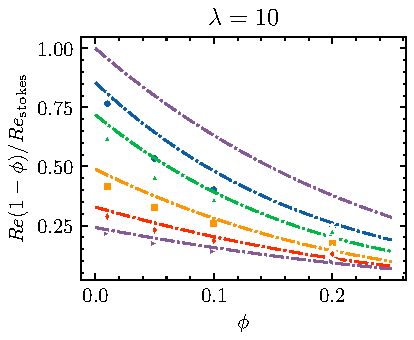
\includegraphics[height = 0.25\textwidth]{image/HOMOGENEOUS_final/CA/U_l_10.pdf}
    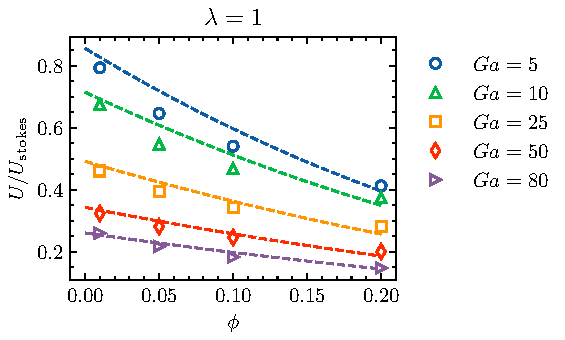
\includegraphics[height = 0.25\textwidth]{image/HOMOGENEOUS_final/CA/U_l_1.pdf}
    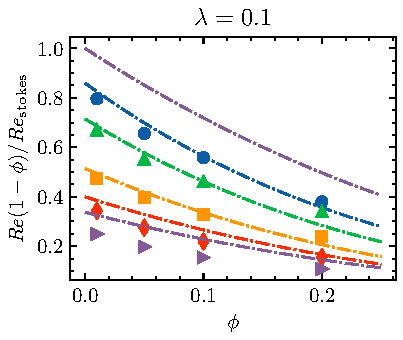
\includegraphics[height = 0.25\textwidth]{image/HOMOGENEOUS_final/CA/U_l_0.pdf}
    \caption{
        Dimensionless rising velocities for (top left) $\lambda  = 10$ (top right) $\lambda =1$ and (bottom) $\lambda = 0.1$. 
        The symbols represents the differents \textit{Galileo} numbers. 
        (dashed lines) Theoretical prediction form \ref{eq:CD0}. 
    }
    \label{fig:drag_force}
\end{figure}




Objectives : 
\begin{itemize}
    \item Present the decomposition of the fluid reynolds stress according to isotropic and deviatoric part.
    \item Show the relation between the flowlines graphs and the actual values of the velocity fluctuation.
    \item Compare our case with \citet{almeras2019fluctuations}
\end{itemize}



We decompose both Reynolds stress into an isotropic part and deviatoric part such that, 
\begin{align}
    \bm{\sigma}^{\text{Re}}_p &=  \rho_d \phi_d K^*_p
    \left[
        \textbf{I}(\textbf{u}_p - \textbf{u}_c)\cdot (\textbf{u}_p - \textbf{u}_c) 
        +\textbf{B}_c \cdot (\textbf{u}_p - \textbf{u}_c)(\textbf{u}_p - \textbf{u}_c)
    \right]\\
    \bm{\sigma}^{\text{Re}}_c &=  \rho_c \phi_c K_c^*
    \left[
        \textbf{I}(\textbf{u}_p - \textbf{u}_c)\cdot (\textbf{u}_p - \textbf{u}_c) 
        +\textbf{B}_p \cdot (\textbf{u}_p - \textbf{u}_c)(\textbf{u}_p - \textbf{u}_c)
    \right]
\end{align}
where the $K^*$ is the dimensionless pseudo-turbulent  kinetic energy, $\textbf{I}$ a unit tensor and $\textbf{B}$ a tensor accounting for the deviation of the Reynolds stress left to determine. 

\subsection{The continuous phase Reynolds stress}
\todo{try \citet{almeras2021statistics} fits}
\todo{also check \citet{almeras2019fluctuations} results}
\tb{might be good to plot the velocity field to examine where does the fluctuation arise (pseudo-turbe or turbe)}
Look at \citep{wang2021numerical} and Mahra.. 2015 



The fluid averaged kinetic energy can be easily scaled on the numerical results shown \ref{fig:Tf_Bf}(left).
\begin{figure}[h!]
    \centering
    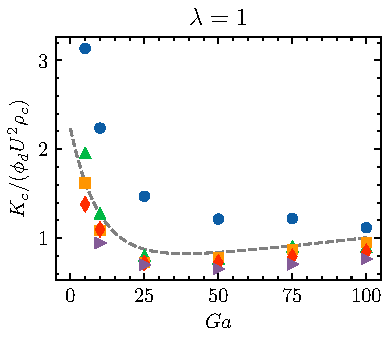
\includegraphics[height=0.3\textwidth]{image/HOMOGENEOUS/fCA/Tf_l_1.pdf}
    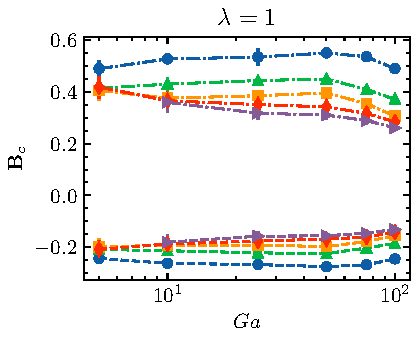
\includegraphics[height=0.3\textwidth]{image/HOMOGENEOUS/fCA/Bf_l_1.pdf}

    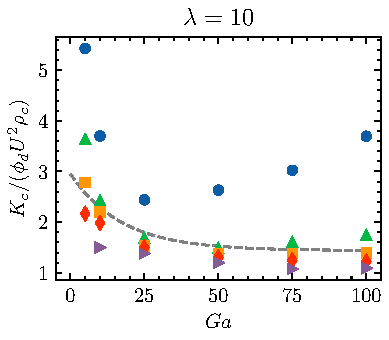
\includegraphics[height=0.3\textwidth]{image/HOMOGENEOUS/fCA/Tf_l_10.pdf}
    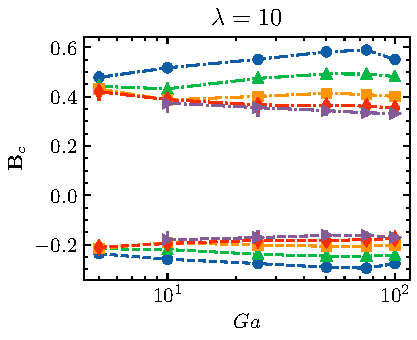
\includegraphics[height=0.3\textwidth]{image/HOMOGENEOUS/fCA/Bf_l_10.pdf}
    \caption{(left) Dimensionless turbulent kinetic energy in terms of the \textit{Galileo} number for different $\phi$. (dots) Numerical simulations, (dashed line) empirical formula \ref{eq:Tf_scaling}.
    The symbols correspond to different volume fraction ($\bullet$) $\phi = 1\%$, ($\blacktriangle$) $\phi = 5\%$, ($\blacksquare$) $\phi = 10\%$, ($\blacklozenge$) $\phi = 15\%$ and ($\blacktriangleright$) $\phi = 20\%$.
    (right) deviatoric part of the Reynolds stress, ($- \cdot -$)  vertical components, $B_{yy}$, ($- -$)  horizontal components, $B_{xx} = B_{zz}$.}
    \label{fig:Tf_Bf}
\end{figure}
\subsection{The particles phase Reynolds stress}

\tb{Maybe include velocity fluctuation and compare to : Lingxin2021 }

\tb{Include Gaussian distribution of bubbles !!! ! ! ! }
Now let's focus on the particular averaged Reynolds stress tensor.
\ref{fig:Talpha_Balpha} shows that the granular temperature behavior is quite similar from the continuous averaged turbulent kinetic energy.
\begin{figure}[h!]
    \centering
    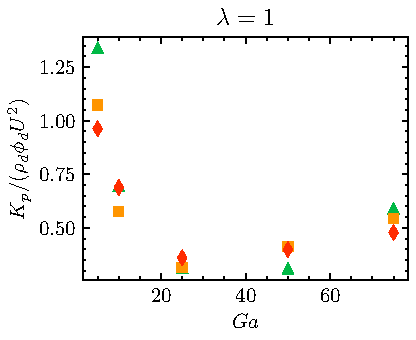
\includegraphics[height=0.3\textwidth]{image/HOMOGENEOUS/fPA/Talpha_l_1.pdf}
    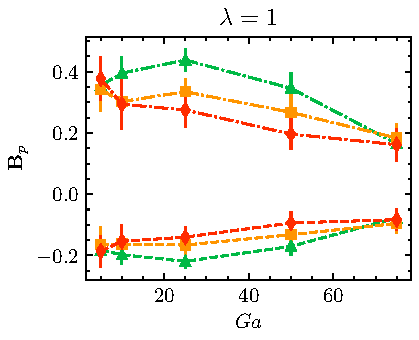
\includegraphics[height=0.3\textwidth]{image/HOMOGENEOUS/fPA/Balpha_l_1.pdf}

    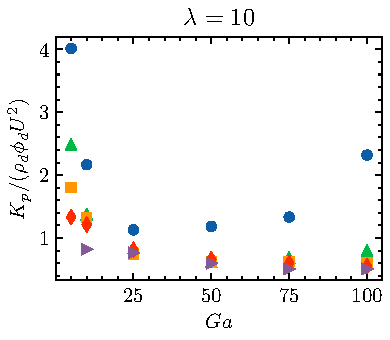
\includegraphics[height=0.3\textwidth]{image/HOMOGENEOUS/fPA/Talpha_l_10.pdf}
    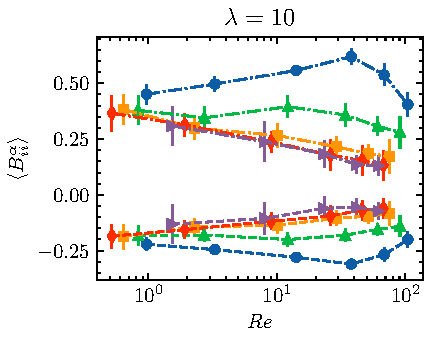
\includegraphics[height=0.3\textwidth]{image/HOMOGENEOUS/fPA/Balpha_l_10.pdf}
    \caption{(left) Dimensionless turbulent kinetic energy in terms of the \textit{Galileo} number for different $\phi$. (dots) Numerical simulations, (dashed line) empirical formula \ref{eq:Talpha_scaling}.
    (right) deviatoric part of the Reynolds stress, ($\bullet$) are the vertical components, $B_{yy}$, ($\blacktriangle$) are the horizontal components, $B_{xx} = B_{zz}$.}
    \label{fig:Talpha_Balpha}
\end{figure}
We can also provide a scaling for the granular temperature, it reads as,  
\begin{equation}
    \frac{\pnavg{T_\alpha}}{U^2}  \approx \frac{\phi}{Ga^2} 2.86\cdot10^{4} 
    \label{eq:Talpha_scaling}
\end{equation}
From \ref{fig:Talpha_Balpha} we observe that this scaling is valid for the lowest \textit{Galileo}. 
The deviatoric part of $\pnavg{T_\alpha}$ is displayed on \ref{fig:Talpha_Balpha}.
It tells us that the Reynolds stress for the particular phase tends to be isotropic in the same way as $\cavg{T}$. 
Indeed, the components of $\pnavg{\textbf{B}}$ go to zero with increasing $Ga$ and $\phi$. 
This behavior is explained by the higher rate of collision present for higher volume fraction and inertia \citep[chapter 1]{jackson2000dynamics}
\subsection{The particle-fluid-particle Stress}
\begin{figure}
    \centering
    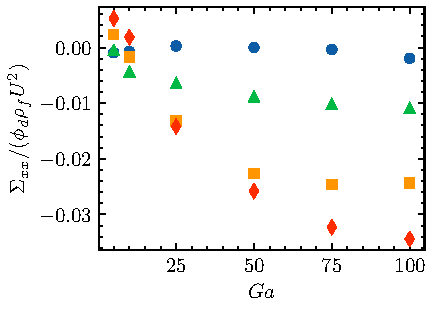
\includegraphics[height=0.3\textwidth]{image/HOMOGENEOUS/fPA/PFPxx.pdf}
    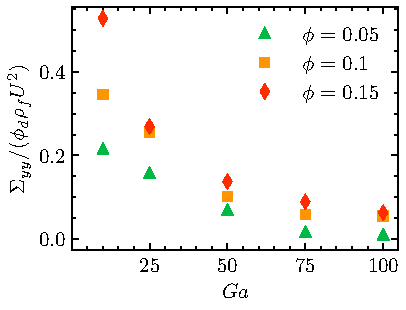
\includegraphics[height=0.3\textwidth]{image/HOMOGENEOUS/fPA/PFPyy.pdf}
    \caption{(left) Normalized PFP stress }
\end{figure}

Open the discussion on the fact that we yet still not have enought data for the pfp stress
\subsection{Higher moments closure : Stresslet ? ? }
\begin{figure}[h!]
    \centering
    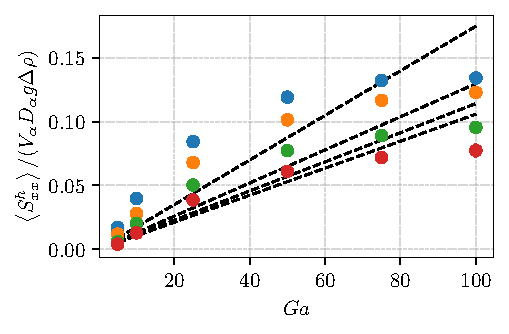
\includegraphics[height=0.3\textwidth]{image/HOMOGENEOUS/fPA/Sxx.pdf}
    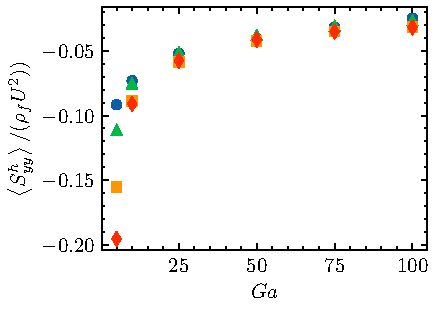
\includegraphics[height=0.3\textwidth]{image/HOMOGENEOUS/fPA/Syy.pdf}
\end{figure}
Lire le papier que JL review 
%%%%%%%%%%%%%%%%%%%%%%%%%%%%%%%%%%%%%%%%%%%%%%%%
%%%%%%%%%%%%%%%%%%%%%%%%%%%%%%%%%%%%%%%%%%%%%%%%
\section{Discussion and conclusion}
We provided statistically representative results for two closure terms and introduce an original numerical methodology.

\section*{Acknowledgement}

\appendix
\section{Space convergence}


Now, let's investigate the required number of droplets per domain, $N_b$, and the minimum definition of cells per diameter of droplets $\delta$.  
\tb{Include bibliography and expectation here \ldots}
For this investigation we kept the physical parameters presented in the same section and made a double parametric analysis over $N$ and $\delta$. 
We carried out simulations for $N = 2, 3, 4, 5, 6, 7$, and for a number of cells $10 <\delta < 40$. 
In Basilisk the mesh definition is defined by a power of two, consequently depending on the size of the domain (which is fixed to keep a $\phi$ constant) the $\delta$ parameter is fixed at a power of 2 close. 
\begin{figure}[h!]
    \centering
    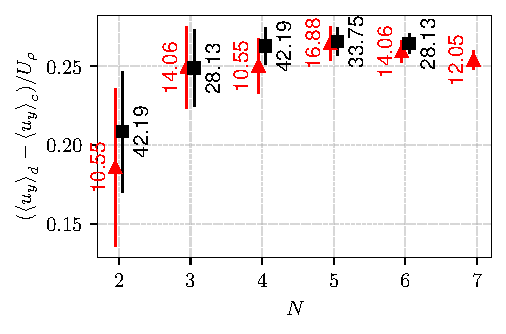
\includegraphics[height= 0.3\textwidth]{image/VALIDATION/N_and_delta/DUd.pdf}
    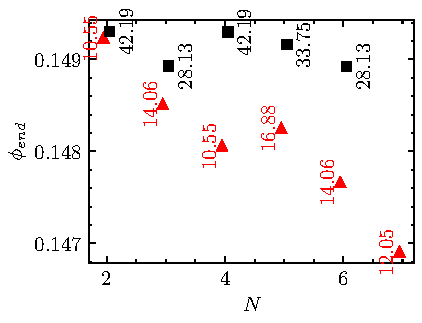
\includegraphics[height= 0.3\textwidth]{image/VALIDATION/N_and_delta/PHI.pdf}
    \caption{(left) Averaged relative velocities for both phases.
            (right) Dispersed phase volume fraction at the end of each simulation.
            The text on the side of the points is $\delta$. }
    \label{fig:VALIDATION_Nd_1}
\end{figure}
\ref{fig:VALIDATION_Nd_1}(left), illustrate clearly that the drift velocity is independent of the parameters $N_b$ and $\delta$, for $N >4$. 
On the other hand, \ref{fig:VALIDATION_Nd_1}(right), show that the volume fraction of the dispersed phase is lower for the low defined grid (red dots), due to a loss of volume during the simulation.
This doesn't mean that the solver isn't volume conservative. 
In fact, it is fund to be due to the \href{http://basilisk.fr/sandbox/fintzin/Rising-Suspension/no-coalescence.h}{no-coalescence.h} which generate fragment into the numerical domain, fragment which are deleted in the long run. 
\begin{figure}[h!]
    \centering
    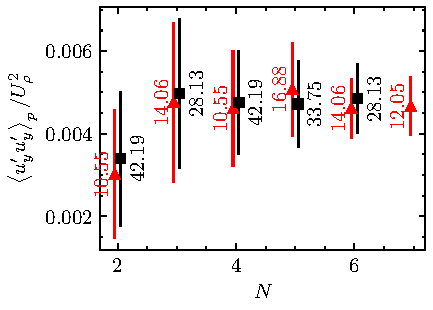
\includegraphics[height= 0.3\textwidth]{image/VALIDATION/N_and_delta/PA_UpUp.pdf}
    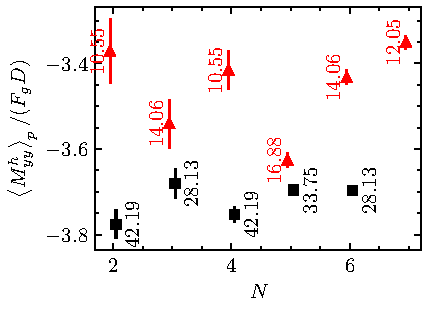
\includegraphics[height= 0.3\textwidth]{image/VALIDATION/N_and_delta/Mh.pdf}
    \caption{(left) Fluids phase averaged fluctuation tensor.
            (right) Particular average of the first moment tensor, where $F_g$ is the buoyancy force applied on one droplet. 
            The numerical values displayed alongside the dots are the number of cells per diameter.}
    \label{fig:VALIDATION_Nd_2}
\end{figure}
Now, let's look at the behavior of more \textit{complicated} closure terms. 
\ref{fig:VALIDATION_Nd_2}(left) demonstrate that the vertical component of the pseudo turbulent tensor is parameter independent rather early, independently of the grid definition. 
This fact is rather surprising but notice that the standard deviation is quite high for small domain. 
On \ref{fig:VALIDATION_Nd_2}(right), we can examine the vertical component of the first moment closure term. 
It is found to be constant for all $N$, but rather inaccurate for coarse grids. 
Which makes sens since the first moment results from a local calculation of the stress over a droplet volume, unlike the other quantities which results from the averaged center of mass velocity of a droplet. 

As we have shown, the quantities presented converge for a number of droplets equivalent to $N = 4$ and $\delta = 25$. 
Thus, we validate our simulation in space, i.e. we made sure that our domain were wide enough to minimize the influence of the periodicity on our results, and in mesh definition. 
Nevertheless, at it is the number of realization that matter when carrying a particular average, it is interesting to look at the duration of the simulation.



\bibliography{Bib/bib_bulles.bib}



\end{document}
